\documentclass{article}

\usepackage{amsmath, amsthm, amssymb, amsfonts}
\usepackage{thmtools}
\usepackage{graphicx}
\usepackage{setspace}
\usepackage[a4paper, top=0in, bottom=1in, left=.5in, right=.5in]{geometry}
\usepackage{float}
\usepackage{hyperref}
\usepackage[utf8]{inputenc}
\usepackage[latvian]{babel}
\usepackage{framed}
\usepackage{microtype}
\usepackage[dvipsnames]{xcolor}
\usepackage{indentfirst}
\usepackage{tcolorbox}
\usepackage{fontspec}
\usepackage{makeidx}
\usepackage{mathtools}
\usepackage{amsmath}
\usepackage{polynom}
\usepackage[T1]{fontenc}     % proper display of accented characters

 
\DeclareMathSizes{10}{12}{8}{6}
\pagestyle{empty}

\graphicspath{{img/}}
\setmainfont{DejaVu Serif}


\colorlet{LightGray}{White!90!Periwinkle}
\colorlet{LightOrange}{Orange!15}
\colorlet{LightGreen}{Green!15}

\newcommand{\HRule}[1]{\rule{\linewidth}{#1}}

\declaretheoremstyle[name=Theorem,]{thmsty}
\declaretheorem[style=thmsty,numberwithin=section]{theorem}
\tcolorboxenvironment{theorem}{colback=LightGray}

\declaretheoremstyle[name=Proposition,]{prosty}
\declaretheorem[style=prosty,numberlike=theorem]{proposition}
\tcolorboxenvironment{proposition}{colback=LightOrange}

\declaretheoremstyle[name=Principle,]{prcpsty}
\declaretheorem[style=prcpsty,numberlike=theorem]{principle}
\tcolorboxenvironment{principle}{colback=LightGreen}

\setstretch{1.2}
\geometry{
    textheight=9in,
    textwidth=5.5in,
    top=1in,
    headheight=12pt,
    headsep=25pt,
    footskip=30pt
}

\makeindex
% ------------------------------------------------------------------------------

\begin{document}

\section{Kompleksie skaitļi}

\subsection{Algebriskais pieraksts}

\subsubsection{Reizināšana}

Skaitļus $3+2i$, $3-2i$ sauc par kompleksi saistītiem.
\begin{equation}
	(a+bi)(a-bi)=a^2-(bi)^2=a^2+b^2
\end{equation}

\subsubsection{Dalīšana}

Izmantojot šo īpašību, kompleksos skaitļus varam iemācīties dalīt.

\begin{equation}
	\frac{a+bi}{x+yi}
	= \frac{(ax+by)(-ay+bx)i}{x^2+y^2}
\end{equation}

\subsubsection{Saknes vilkšana}

Kvadrāsakni no algebriskā pierakstā rakstītiem kompleksiem skaitļiem var vilkt ar formulu:
\begin{equation}
	\sqrt{a+bi}=\pm
	\left(
	\sqrt{\frac{\sqrt{a^2+b^2}+a}{2}+\beta i\sqrt{\frac{\sqrt{a^2+b^2}-a}{2}}}
	\right)
\end{equation}

\subsubsection{Kompleksā plakne}

Kompleksos skaitļus algebriskā pierakstā varam attēlot kompleksajā planknē.

\begin{figure}[!htb]
	\centering
	\caption{Kompleksā plakne}
	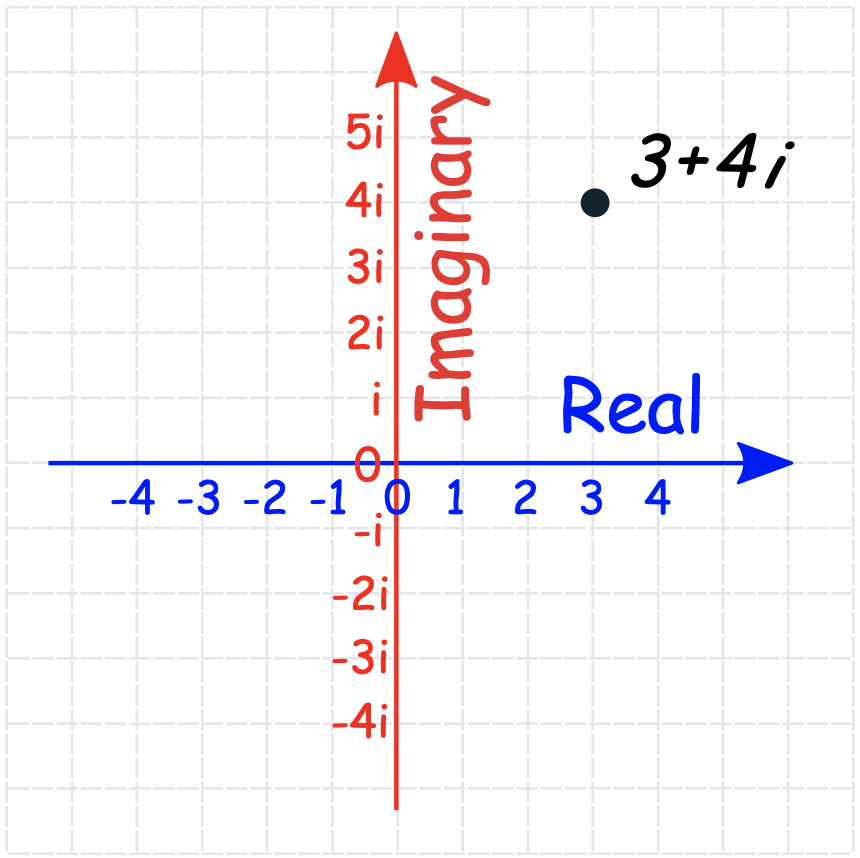
\includegraphics[width=.3\linewidth]{complex_plane-1}
\end{figure}

\subsection{Trigonometriskais pieraksts}

\subsubsection{Definīcija}

Kompleksu skaitli $z =a+bi$ kā plaknes punktu var uzdot arī ar: polāro rādiusu $r$ (skaitļa moduli, jeb absolūto vērtību, $r=|z|$) un polāro leņķi $\varphi$ (skaitļa argumentu, $\varphi=arg(z)$).
\begin{figure}[!htb]
	\centering
	\caption{Polārās koordinātas}
	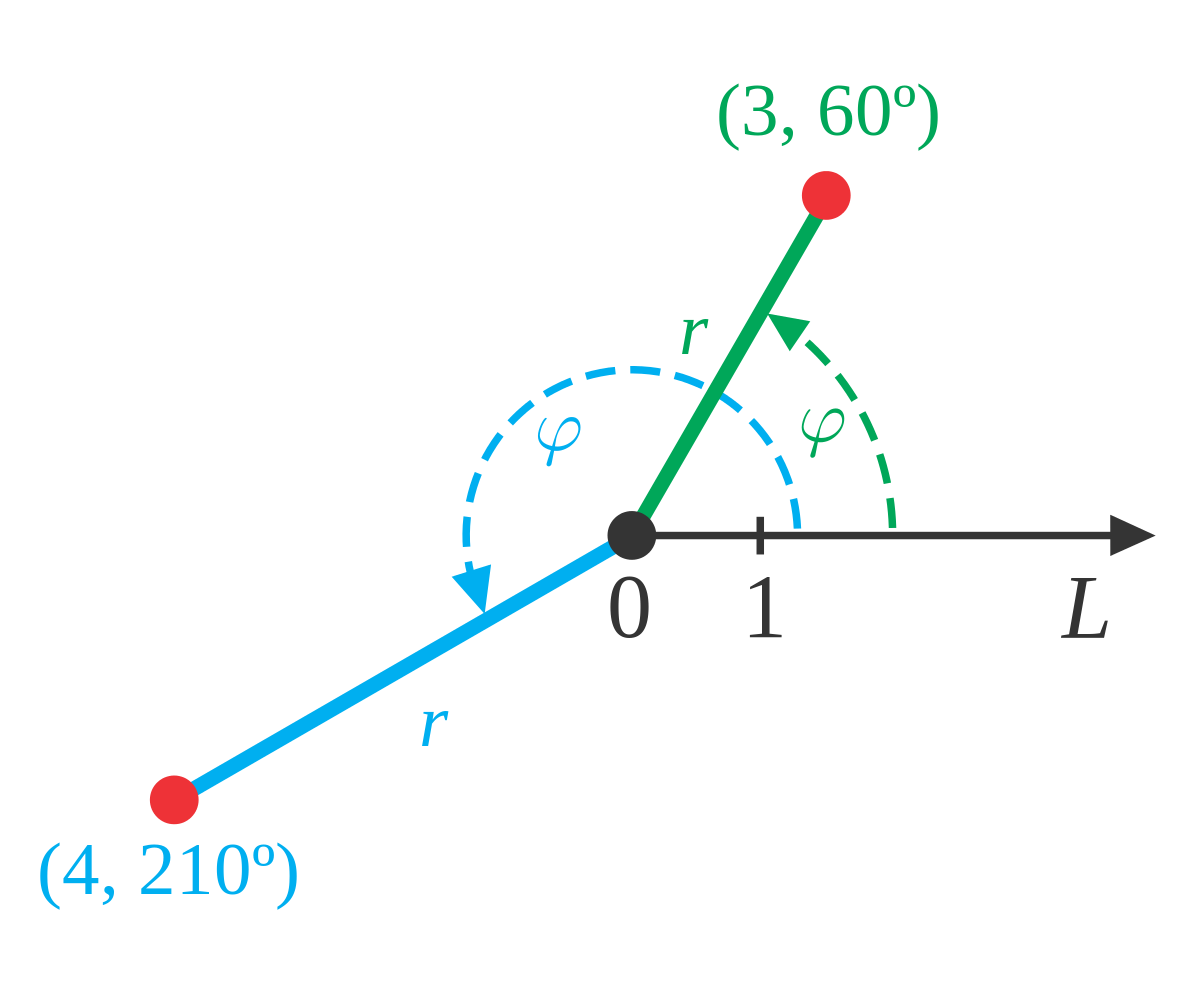
\includegraphics[width=0.3\linewidth]{polar_coordinates-1}
\end{figure}

Moduļa aprēkināšana:
\begin{equation}
	r=\sqrt{a^2+b^2}
\end{equation}

\subsubsection{Reizināšana}

Reizinot divus kompleksus skaitļus, trigonometriskajā pierakstā
viss sanāk ļoti vienkārši un simetriski:
\begin{equation}
	zz'=rr'(\cos(\varphi+\varphi')+i\sin(\varphi+\varphi'))
\end{equation}

\textbf{Teorēma.} Komplekso skaitļu reizinājuma modulis ir reizinātāju moduļu reizinājums, bet reizinājuma arguments - reizinātāju argumentu summa.

\subsubsection{Dalīšana}

Pieņemsim, ka skaitlis z' nav 0. Tad:
\begin{equation}
	\frac{z}{z'}=\frac{r}{r'}(\cos(\varphi-\varphi')+i\cos(\varphi-\varphi'))
\end{equation}


\subsubsection{Kāpināšana}

Ja $n>1$, tad $z^n$ apzīmē $z\cdot\ldots\cdot z$ (n reizes).

\textbf{Teorēma:} Ja $m,n>1$, tad:

\begin{align}
	&z^m z^n = z^{m+n}; \\
	&(z^m)^n=z^{mn}
\end{align}


\subsubsection{Muavrā formula (kāpināšana trigonometriskajam pierakstam)}

\begin{equation}
	r(\cos(\varphi) = i\sin(\varphi))^n=r^n(\cos(n\varphi)+i\sin(n\varphi))
\end{equation}

\subsubsection{Saknes vilkšana}

\textbf{Teorēma.} Ja kompleksais skaitlis
\begin{equation}
	z = R(\cos\varPhi + i \sin \varPhi)
\end{equation}
nav 0, tad saknei $\sqrt[n]{z}$ ir tieši $n$ dažādas vērtības, un tās var iegūt no formulas:

%TK saknes vilkšanas formula

\section{Polinomi}

\subsection{Definīcijas}

Iespējami divi polinomu vienādības jēdzieni:
\begin{itemize}
	\item Teiksim, ka polinomi $P1(x)$ un $P2(x)$ ir vienādi kā izteiksmes, ja to kanoniskie pieraksti satur vienādas x pakāpes un vienādus koeficientus pie attiecīgajām x pakāpēm.
	\item Teiksim, ka polinomi $P1(x)$ un $P2(x)$ ir vienādi kā funkcijas, ja visiem kompleksiem skaitļiem x, $P1(x)$ = $P2(x)$.
\end{itemize}

\textbf{Teorēma.} Ja polinomi ir vienādi kā izteiksmes, tad tie ir vienādi arī kā funkcijas.

\textbf{Teorēma.} Ja polinomi ir vienādi kā funkcijas, tad tie ir vienādi arī kā izteiksmes (t.i. tiem ir vienādi kanoniskie pieraksti).

\subsection{Saskaitīšana}

\textbf{Teorēma.} Polinomu summas pakāpe:
\begin{itemize}
	\item ja $deg(P)<deg(Q)$, tad $deg(P+Q)=deg(Q)$;
	\item ja $deg(P)=deg(Q)$, tad $deg(P+Q) \le deg(Q)$.
\end{itemize}

\subsection{Reizināšana}

\textbf{Teorēma.} Nenulles polinomu reizinājuma pakāpe ir vienāda ar reizināmo pakāpju summu:

\begin{equation}
	deg(PQ) = deg(P)+deg(Q)
\end{equation}

\subsection{Dalīšana}

\textbf{Teorēma.} Dalīšanu $\frac{1}{P}$ var izpildīt tad un tikai tad, ja $P$ ir nulltās pakāpes polinoms.


\textbf{Teorēma.} Jebkuriem diviem polinomiem $P(x)$ un $Q(x)$, ja $Q$ nav nulles polinoms, tad var atrast vienīgos polinomus - dalījumu $D(x)$ un atlikumu $R(x)$ tādus, ka $P(x)=Q(x)D(x)+R(x)$, un $R(x)$ pakāpe ir mazāka par dalītāja $Q(x)$ pakāpi vai arī $R(x)$ ir nulles polinoms.

\textbf{Teorēma.} Ja $P(x)$ dalās ar $Q(x)$, un $Q(x)$ dalās ar $R(x)$, tad arī $P(x)$ dalās ar $R(x)$.
\textbf{Teorēma.} Ja $P(x)$ un $Q(x)$ abi dalās ar $R(x)$, tad arī $P(x)+Q(x)$ un $P(x)−Q(x)$ dalās ar $R(x)$.
\textbf{Teorēma.} Ja $P(x)$ dalās ar $R(x)$, tad jebkuram $Q(x)$ reizinājums $P(x)Q(x)$ arī dalās ar $R(x)$.

\textbf{Teorēma.} Jebkurš polinoms dalās ar jebkuru nulltās pakāpes polinomu.

\textbf{Teorēma.} Ja $P(x)$ dalās ar $Q(x)$, tad tas dalās arī ar $cQ(x)$, kur $c$ – jebkurš skaitlis, kas nav $0$.

\textbf{Teorēma.} Ja $P$ un $Q$ pakāpes ir vienādas, tad $P(x)$ dalās ar $Q(x)$ tad un tikai tad, ja $Q(x)=cP(x)$, kur $c$ – skaitlis, kas nav $0$.

\textbf{Teorēma.} Ja $c$ – skaitlis, kas nav $0$, tad polinomiem $P(x)$ un $cP(x)$ ir vieni un tie paši dalītāji.

\subsubsection{Piemērs}

\resizebox{0.8\linewidth}{!}{\polylongdiv[style=C]{x^6 - x^4 + x^3 - 2x^2 + 5x - 9}{x^3 - 3x + 4}}



\subsection{Lielākais kopīgais dalītājs}
\subsubsection{Definīcija}
\textbf{Def. }Polinomus mēs nevaram sakārtot pēc "lieluma". Kaut kādu sakārtojumu dod tikai polinomu pakāpes.  Tāpēc mēģināsim definēt divu polinomu lielāko kopīgo dalītāju (LKD, jeb angliski - GCD, greatest common divisor) kā kopīgo dalītāju ar visaugstāko pakāpi.

\textbf{Bet:} ja $D(x)$ ir divu polinomu kopīgs dalītājs, tad tāds ir arī $cD(x)$. Tāpēc būs lietderīgi vienoties, ka “oficiālā” lielākā kopīgā dalītāja koeficients pie lielākās $x$ pakāpes ir 1.

\subsubsection{''Gausa'' metodes piemērs}

\textbf{Piemērs.}
\begin{equation}
	P(x)=x3-6x2+11x-6; Q(x)=x2-7x+10.
\end{equation}
Pakāpju summa ir 5.

\textbf{Pirmais solis} - likvidējam $x^3$: 
\begin{equation}
	P1=P-xQ=x2+x-6.
\end{equation}
Šeit koeficients pie x2 ir 1, tāpēc papildus apsvērums nav jāpiemēro.  Saskaņā ar Lemmu, pārim \\ ${x2+x-6, x2-7x+10}$ ir tie paši kopīgie dalītāji, kas pārim {P, Q}, bet tā pakāpju summa ir 4.

\textbf{Otrais solis} - likvidējam vienu no x2:
\begin{equation}
	P2=P1 - Q =(x2+x-6)-(x2-7x+10)=8x-16.
\end{equation}
Piemērojam minēto papildus apsvērumu, un izdalām ar 8, iegūstot: $P2=x - 2$.  Saskaņā ar lemmu, pārim ${x-2, x2-7x+10}$ ir tie paši kopīgie dalītāji, kas pārim {P, Q}, bet tā pakāpju summa ir 3.

\textbf{Trešais solis} - likvidējam atlikušo x2:
\begin{equation}
	P3=Q-xP2=( x2 - 7 x +10)- x( x - 2)=-5 x+10 .
\end{equation}
Piemērojam papildus apsvērumu, un izdalām ar -5, iegūstot: $P3=x - 2$ .
Pārim ${x-2, x-2}$ ir tie paši kopīgie dalītāji, kas pārim ${P, Q}$,
bet tā pakāpju summa ir 2.  Bet pāra ${x-2, x-2}$ LKD ir $x-2$, tāpēc arī $LKD(P, Q)=x-2$:
\begin{equation}
	LKD(x3-6x2+11x-6, x2-7x+10)=x-2.
\end{equation}

Pārim ${x-2, x-2}$ ir tikai divu veidu kopīgie dalītāji: skaitļa 1 daudzkārtņi un polinoma x-2 daudzkārtņi. Tātad visi šie kopīgie dalītāji ir arī LKD dalītāji.  Šis process varēja beigties arī ātrāk, ja tiktu iegūts pāris ${0, R}$.  Šāda pāra LKD ir $R$, tas tad būs arī pāra ${P, Q}$ LKD.  Bet process varēja beigties arī ar pāri ${a, b}$, kur $a, b$ abi ir skaitļi.  Tas tad nozīmētu, ka polinomu ${P, Q}$ LKD ir null-tās pakāpes polinoms 1:
\begin{equation}
	LKD(P, Q)=1.
\end{equation}


\subsection{Polinomu būvēšana}

\subsubsection{Dabiskā metode}

Tikko pierādījām, ka ja pakāpei ir jābūt ne lielākai par n, tad tāds polinoms var būt tikai viens. Piemērs. Uzbūvēt polinomu P(x) tādu, ka P(1)=3; P(2)=-2; P(3)=2.

Doti 3 punkti, $3=2+1$, tātad tas būs kvadrātisks polinoms $y=ax^2+bx+c$.
Dabiska metode - sastādām 3 lineāru vienādojumu sistēmu:

\begin{align}
	&P(1)=a+b+c=3 \\
	&P(2)=4 a+2 b+c=-2 \\
	&P(3)=9 a+3 b+c=2.
\end{align}

To atrisinot, iegūstam: a=$\frac{9}{2}$ ; $b=\frac{-37}{2}$; $c=17$ , tātad meklētais polinoms ir: $P(x)=\frac{9}{2} x^2 +\frac{-37}{2}x+17$ 

\subsubsection{Vandermonda matrica (vispārīgi)}

Vispārīgais gadījums: mēs gribam uzbūvēt n-ās (vai zemākas) pakāpes polinomu;
\begin{equation}
	P(x)=a_n+ x_n +a_{n-1}x^{n-1} +\ldots +a_1x+a_0
\end{equation}
kas $n+1$ punktos $x_1 , x_2 ,... , x_n , x_{n+1}$ pieņem dotās vērtības $y_1 , y_2 , ... , y_n , y_{n+1} $.
No prasītajām $n+1$ vienādībām $(i=1..n+1)$:
\begin{equation}
	P(x_i)=a_nx_i^n+a_{n-1}+x_i^{n-1} +\ldots+a_1x_i+a_0= y_i
\end{equation}
iegūstam $(n+1)\times(n+1)$ lineāru vienādojumu sistēmu, kuras atrisināšana dos polinoma koeficientu $a_j$ vērtības:

\begin{center}
	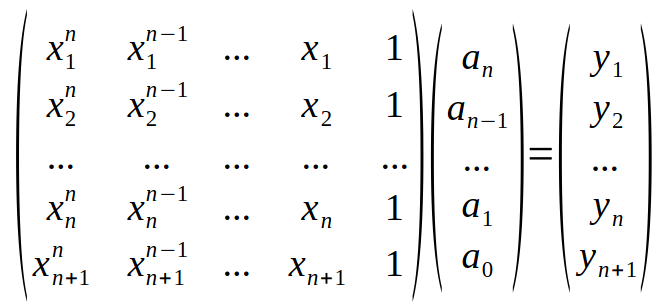
\includegraphics[width=0.5\linewidth]{Vandermond_matrix-1}
\end{center}

\section{$\mathbb{Z}$ Lauki (un gredzeni)}

\subsection{Nulles dalītāji}

\textbf{Def.} Gredzenā G divus nenulles elementus a, b, kam a*b=0, sauksim par nulles dalītājiem.

\subsection{Inversie elementi}

\textbf{Def.} Gredzena elementam a mēs varam nodefinēt apgriezto elementu (jeb inverso elementu) kā vienādojumu $xa=ax=1$ atrisinājumu.
Laukā katram elementam eksistē tā inversais elements.

\subsection{Saskaitīšanas tabula $\mathbb{Z}_7$}

\begin{tabular}{c|ccccccc}
+ & 0 & 1 & 2 & 3 & 4 & 5 & 6 \\ \hline
0 & 0 & 1 & 2 & 3 & 4 & 5 & 6 \\
1 & 1 & 2 & 3 & 4 & 5 & 6 & 0 \\
2 & 2 & 3 & 4 & 5 & 6 & 0 & 1 \\
3 & 3 & 4 & 5 & 6 & 0 & 1 & 2 \\
4 & 4 & 5 & 6 & 0 & 1 & 2 & 3 \\
5 & 5 & 6 & 0 & 1 & 2 & 3 & 4 \\
6 & 6 & 0 & 1 & 2 & 3 & 4 & 5 \\
\end{tabular}


\subsection{Reizināšanas tabula $\mathbb{Z}_7$}

\begin{tabular}{c|ccccccc}
$\times$ & 0 & 1 & 2 & 3 & 4 & 5 & 6 \\ \hline
0 & 0 & 0 & 0 & 0 & 0 & 0 & 0 \\
1 & 0 & 1 & 2 & 3 & 4 & 5 & 6 \\
2 & 0 & 2 & 4 & 6 & 1 & 3 & 5 \\
3 & 0 & 3 & 6 & 2 & 5 & 1 & 4 \\
4 & 0 & 4 & 1 & 5 & 2 & 6 & 3 \\
5 & 0 & 5 & 3 & 1 & 6 & 4 & 2 \\
6 & 0 & 6 & 5 & 4 & 3 & 2 & 1 \\
\end{tabular}

\subsection{Dalīšanas tabula $\mathbb{Z}_7$}

\begin{tabular}{c|ccccccc}
$\div$ & 1 & 2 & 3 & 4 & 5 & 6 \\ \hline
0 & 0 & 0 & 0 & 0 & 0 & 0 \\
1 & 1 & 4 & 5 & 2 & 3 & 6 \\
2 & 2 & 1 & 6 & 4 & 5 & 1 \\
3 & 3 & 6 & 1 & 5 & 2 & 4 \\
4 & 4 & 2 & 4 & 1 & 6 & 5 \\
5 & 5 & 3 & 2 & 6 & 1 & 4 \\
6 & 6 & 5 & 3 & 4 & 2 & 1 \\
\end{tabular}


\end{document}